\section{AIS Trade Flow System}

AIS Trade Flow systems utilize data transmitted by vessels worldwide to furnish both real-time and historical insights into maritime trade operations \autocite{halden2019estimation}. 
The primary aim is to establish a framework that delineates trade activities between ports, leveraging AIS signals. 
Designating port areas within AIS Trade Flow systems is a multifaceted undertaking encompassing geographical and operational factors. 
From a geographical perspective, a port area is typically demarcated by a set of coordinates outlining the physical confines of the port and its adjacent waters. 
This encompassing region might encompass berths, anchorages, and at times, even approach channels. Identifying whether a ship resides within a port area often necessitates comparing its current AIS-reported coordinates with the established port boundaries. 
Should the ship's location fall within these boundaries, it's deemed situated within the port area. 
Nonetheless, the analysis transcends mere geographical coordinates. 
For instance, a ship might exist within a port's geographical bounds; 
however, if it's merely passing through without halting or participating in port operations, it might not qualify as being `in port` from an operational standpoint.

Addressing these intricacies, AIS Trade Flow systems frequently employ advanced algorithms to precisely ascertain port boundaries and classify vessel conduct. 
This assessment takes into account parameters like the vessel's velocity, heading, and historical behavioral trends. 
Through the integration of these diverse data facets, these systems can render an exceptionally precise portrayal of port undertakings and vessel trajectories. 
AF Code has constructed such a system by adhering to overarching principles, resulting in the creation of a dataset incorporating AIS signals alongside information about port visits, cargo loading, and unloading.



\begin{figure}[h]
    \centering
    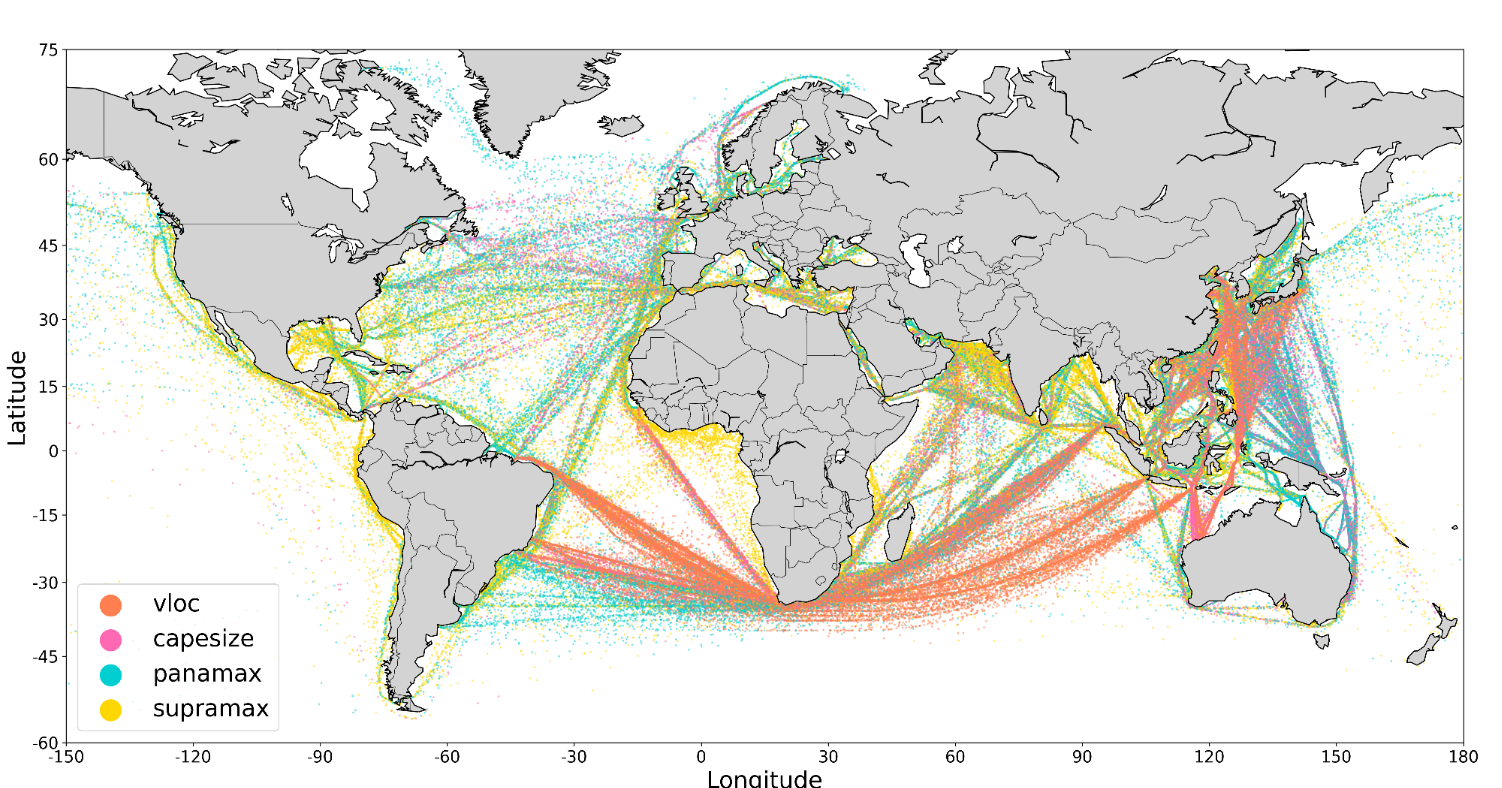
\includegraphics[width=0.7\textwidth]{images/tradeflow_system.png}
    \caption{Trade flow from 150,000 AIS sampled signals.}
    \label{tradeflow_system}
\end{figure}

To achive this, the AIS data is processed to identify port-to-port voyages and then stored them in a database based on segments as shown in the Figure \ref{ais_processing}

\begin{figure}[h]
    \centering
    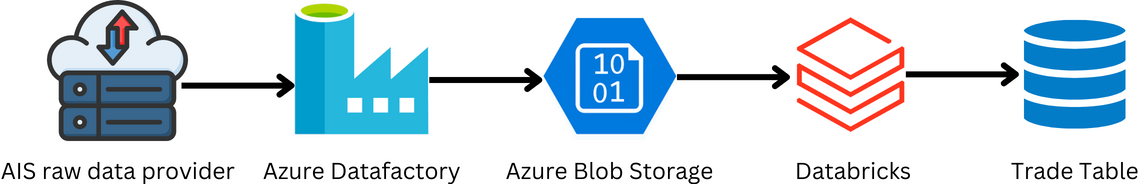
\includegraphics[width=0.8\textwidth]{images/ais_processing.png}
    \caption{AIS Raw Data Processing}
    \label{ais_processing}
\end{figure}

\subsection{Vessel Voyages}

Trade flow systems are designed to identify port-to-port voyages. 
Each of this voyages is either Laden voyage or Ballast voyage from one port to another. 
At port vessel can load or unload cargo or just refuel and continue to another port.
It is important to determine port stops and port area to identify the type of voyage.
This section will describe how these voyages are identified and classified. 


\subsubsection{Laden Voyages}

The laden voyage concept centers on cargo movement, distinct from the vessel's own traversal. 
This characterization holds particular significance in evaluating logistical chains and cargo dynamics within maritime transportation. 
A laden voyage pertains to the route spanning from the cargo's loading point at the departure port to its unloading point at the arrival port. 


\subsubsection{Ballast Voyages}

The ballast voyage concept centers on the vessel's movement without cargo, contrasting with its movement when laden. 
A ballast voyage is characterized as the route from the port of cargo unloading, serving as the departure port, to the port of cargo loading, functioning as the arrival port.

\subsection{Port Stop and Port Area}

The initial key phase involves obtaining the coordinates of the targeted port and subsequently establishing a polygon encompassing its vicinity. 
The overarching approach revolves around quantifying unique visits within this polygon, using a geo-fence strategy. 
Given the utilization of S-AIS data, there exist temporal intervals during which satellites may not receive ship messages due to blind zones. 
This introduces the potential for ships to enter and exit the designated port area without satellite detection. 
To mitigate this, a larger polygon around the port can decrease the likelihood of overlooked visits. However, such an expansive polygon could result in the inclusion of vessels merely passing through, particularly if the port is positioned near a major shipping route. 
Hence, the ideal polygon size is contingent on the port's location, it should be sizable enough to capture all visits yet sufficiently compact to exclude vessels in transit. 
This is illustrated by Figure \ref{port_area}, showcasing LNG terminals in Trinidad and Algeria enclosed by identical polygons.
Visual inspection reveals message flow towards the port in Trinidad (5.4a) and a substantial portion of vessel flow bypassing the port in Algeria (5.4b). 
Additionally, supplementary criteria like capping maximum speed and requiring navigational statuses of $anchored$ or $moored$ can be incorporated to ensure vessels are genuinely engaged in loading activities \autocite{halden2019estimation}.

\begin{figure}[h]
    \centering
    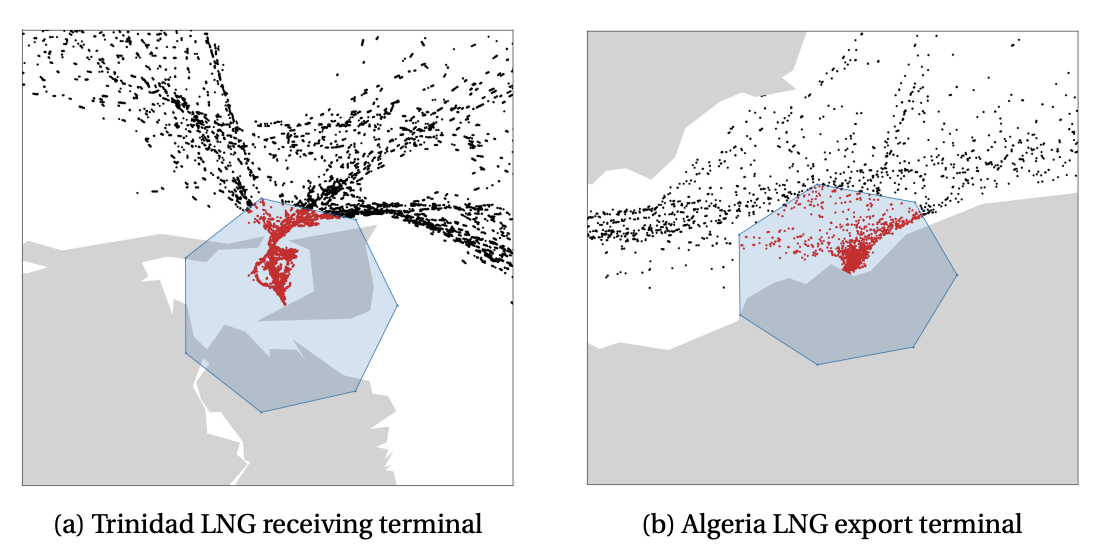
\includegraphics[width=0.8\textwidth]{images/port_area.png}
    \caption{Port Area}
    \label{port_area}
\end{figure}

By using the trade flow system described in this section, we can figure out the trades made by ships in 2022. 
If we assume that these ships will continue with the same trading patterns in 2023, we can use the trade data to make an estimate of emissions for 2023.